% !TEX root = main.tex
We consider an off-line scenario, which means we know all $t_i$'s and $\ETx_i$'s, non causally. We assume that the receiver harvests energy only once (say of amount $E$) at time $r_0=0$. Hence, the receiver (and so does the transmitter) can be \textit{on} for a maximum period of $\TRx_0=\frac{E}{P_r}$. We also assume that an infinite battery capacity is available both at the transmitter and the receiver to store the harvested energy. Our objective is to complete transmission (transmit $B_0$ bits) as early as possible. This is stated as an optimization problem below.

%The transmitter is supposed to transmit all $B_0$ bits in as minimum time as possible. The problem is formally stated below.
\begin{problem}
\begin{align}
&\min_{\{\textbf{p},\textbf{s},N\}}			&& T
\\
&\text{subject to} 				&& B(T)=B_0, 
\label{pb1_constraint_bits}
\\
&     										&& U(t)\le \mathcal{E}(t)  		&&& \forall \; t\;\in\;[0,T], \label{pb1_constraint_energy}
\\
&    										&& s_{N+1}-s_1\le \TRx_0.
\label{pb1_constraint_time}
\end{align}
\end{problem}
Constraint \eqref{pb1_constraint_energy} means that we cannot use more than available energy at any point of time till we finish transmission. \eqref{pb1_constraint_time} implies that the maximum duration of transmission cannot exceed $\TRx_0$. Note that the maximum transmission duration is actually given by $\displaystyle\sum_{i=1:p_i\neq 0}^{N}(s_{i+1}-s_i)$, but as we shall see in Lemma \ref{lemma_nobreaks}, this reduces to $(s_{N+1}-s_1)$.  

Before describing an algorithm to solve Problem 1, we state the following Lemmas, which shall help us construct our algorithm.
% !TEX root = OptimalOffline.tex

\begin{lemma}
The transmission power in an optimal solution $\{\textbf{p},\textbf{s},N\}$ to Problem 1 is non-decreasing with time whenever the receiver is '\textit{on}' i.e. $p_i\ge p_j$ for all $i\in \{1,2..N\},j<i$ if $p_i\neq 0$. 
\label{lemma_increasing_power}
\end{lemma}
\begin{proof}
We prove this by contradiction. Assume that the optimal solution $\{\textbf{p},\textbf{s},N\}$ does not follow the condition stated in Lemma \ref{lemma_increasing_power}. Let $i$ be the minimum index for which the condition is violated. So, $\exists j<i:\ p_i<p_j $. Let $j$ be the maximum index less than $i$ such that $p_i<p_j$. 

%
%\begin{lemma}
%The transmission power in every optimal solution to Problem 1 is non-decreasing with time whenever the receiver is \textit{on}.
%\label{lemma_increasing_power}
%\end{lemma}
%\begin{proof}
%We prove this by contradiction. The following two cases arise depending on whether the receiver is \textit{on} or \textit{off}.

$Case 1:$ Suppose $j=i-1$. This situation is shown in Fig. \ref{Lemma1}. In this case consider a new transmission policy which is same as the optimal policy till time $s_{i-1}$. From $s_{i-1}$ to $s_{i+1}$ this new policy transmits at a constant power $p'=\dfrac{p_i(s_{i+1}-s_{i})+p_{i-1}(s_{i}-s_{i-1})}{s_{i+1}-s_{i-1}}$. Then the number of bits transmitted in this new policy till $s_{i+1}$ would be more than the optimal policy, due to concavity of $g(p)$ as shown below.
\begin{align*}
&g(p_i)\frac{s_{i+1}-s_{i}}{s_{i+1}-s_{i-1}}+g(p_{i-1})\frac{s_{i}-s_{i-1}}{s_{i+1}-s_{i-1}}
\\ 
&\le g\left(\frac{p_i(s_{i}-s_{i-1})+p_{i-1}(s_{i+1}-s_{i})}{s_{i+1}-s_{i-1}}\right),
\\
&\implies g(p')(s_{i+1}-s_{i-1})
\\
&\ge g(p_i)(s_{i+1}-s_{i})+g(p_{i-1})(s_{i}-s_{i-1}).  
\end{align*}
After time $s_{i+1}$, the policy that we are describing follows same transmission powers as the optimal policy till it transmits $B_0$ bits. Since the policy has transmitted more number of bits than the optimal policy till time $s_{i+1}$, it would finish transmitting all $B_0$ bits at an earlier time than the optimal policy. Hence, this new policy contradicts the optimality of policy $\{\textbf{p},\textbf{s},N\}$.

$Case 2:$ When $j<i-1$, by our assumption on choosing $j$, $p_i>p_{i-1},..,p_{j+1}$ and $p_i<p_{j}$. As $i$ is the minimum index violating the condition stated in Lemma \ref{lemma_increasing_power}, we can argue that $p_{i-1},..,p_{j+1}=0$. This situation is shown in Fig. \ref{Lemma1}. Now, consider a policy where the transmission power is same as the optimal policy before time $s_j$ and after time $s_{i+1}$. From $s_j$ to $s_j'=s_j+s_{i}-s_{j+1}$ the policy keeps the receiver \textit{off} and from $s_j'$ to $s_{i}$ it transmits at power $p_j$. This policy still transmits same number of bits and ends at the same time as the optimal policy. This policy matches with the form of optimal policy in \textit{Case1}. From this policy we can generate another policy which would finish earlier than the optimal policy as we did is \textit{Case1} and reach a contradiction. 
\end{proof}

\begin{figure}[htb]
  \centering
  \centerline{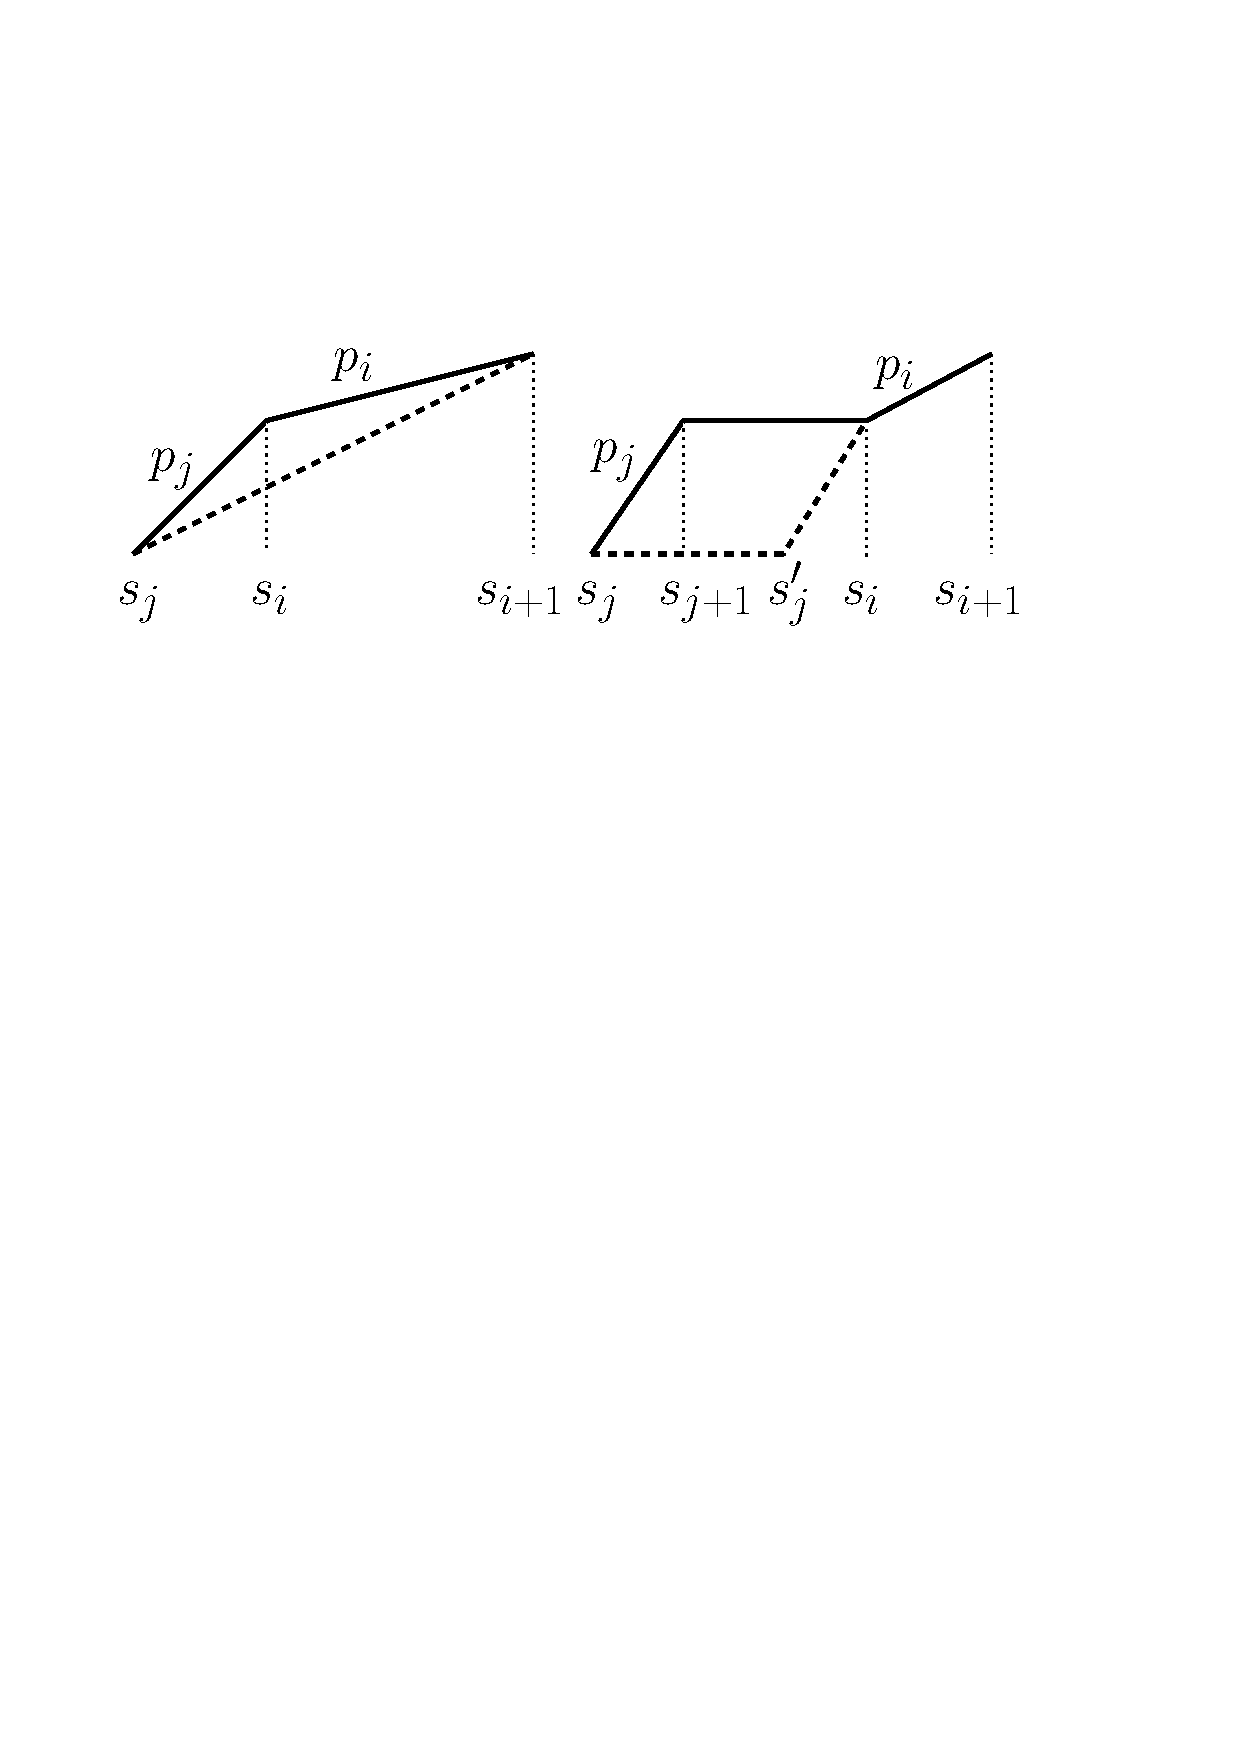
\includegraphics[width=8cm]{Lemma1.pdf}}
\caption{Figure showing the two cases of Lemma \ref{lemma_increasing_power}, \textit{Case 1} (left)  and \textit{Case2} (right) with $p_i>p_j$.}\label{Lemma1}
\end{figure}

\begin{lemma}
The optimal solution to Problem 1 may not be unique, but there always exists an optimal solution where once transmission has started, the receiver remains '\textit{on}' until the transmission is complete. \label{lemma_nobreaks}
\end{lemma}
\begin{proof}
The proof involves showing that we can generate an optimal solution with no breaks in transmission from any other optimal solution. Let the optimal policy be $\{\textbf{p},\textbf{s},N\}$. Now, if $p_i\neq 0,\forall \ i$, then we are done. Suppose some of $p_i$'s, say $p_{i_1},p_{i_2},...,p_{i_k}=0$ for some $k<N$, where $i_1<i_2<..<i_k$. Let $p_j$ be the first non-zero power after $p_{i_1}$. Consider a new policy which is same as policy $\{\textbf{p},\textbf{s},N\}$ till time $s_{i_1-1}$ and after time $s_{j}$. But, it keeps the receiver \textit{off} for a period of $(s_{j}-s_{i_1})$ starting from time $s_{i_1-1}$ and transmit with power $p_{i_1-1}$ from time $s_j'=(s_{i_1-1}+s_{j}-s_{i_1})$ till $s_j$. This policy transmits same amount of bits in same time as policy $\{\textbf{p},\textbf{s},N\}$ and also satisfies all constraints. So this policy is also optimal. But, in this policy the receiver \textit{off} duration, $(s_{j}-s_{i_1})$, has been shifted to left as shown in Fig.\ref{fig_Lemma2} (a). We continue this process of shifting the receiver \textit{off} period to left again and again to generate new optimal  policies till we reach a policy where the receiver is \textit{off} for time $(s_{j}-s_{i_1})$ from $s_1$ as shown in Fig. \ref{fig_Lemma2} (b). The start time of this policy (the one showed with solid line in Fig. \ref{fig_Lemma2} (b)) can now be changed to $s_1'=(s_1+s_{j}-s_{i_1})$. 

Similarly, we shift the receiver \textit{off} period corresponding to $p_{i_2},...,p_{i_k}$ till the total \textit{off} period is shifted to the beginning of transmission. This will result in a policy which starts after time $s_1$ and ends at time $s_{N+1}$, but the transmission power never goes zero in-between. Such a policy is also optimal and has no breaks.
\end{proof}
\begin{figure}[htb]
  \centering
  \centerline{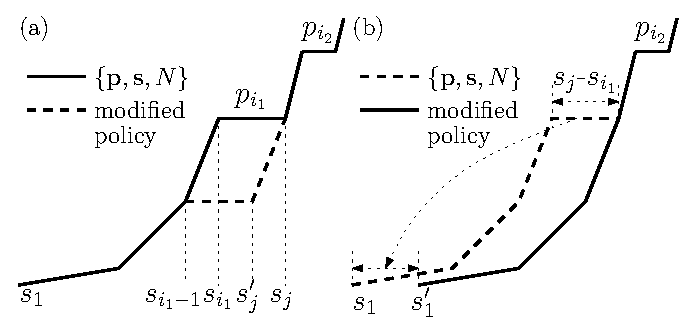
\includegraphics[width=8cm]{Lemma2.eps}}
\caption{Illustration of Lemma \ref{lemma_nobreaks}. Receiver \textit{off} time of $s_{j}-s_{i_1}$ is progressively shifted to left as shown in (a) to (b).}\label{fig_Lemma2}
\end{figure}
In rest of the paper, whenever we refer to the optimal solution for Problem 1, we assume it is the one with no breaks in transmission.
%This is equivalent to saying that there are no breaks during transmission in an optimal solution. Again, we shall prove this by contradiction. In the optimal solution, suppose the receiver is \textit{off} for some period after transmission starts. Let the transmission power before the break is $p_1$ and after the break is $p_2$. Considering Lemma \ref{lemma_increasing_power}, $p_1<p_2$, as shown in Fig. \ref{Lemma2_figure} (a). Consider the policy where we keep the receiver \textit{off} from time $A$ to $B'=(A+C-B)$. Now, an energy arrival can occur at the transmitter at any time between $A$ to $D$. If there is no energy arrival then transmitting at a constant rate from $B'$ to $D$ would transmit more bits.
%
%$Case 1:$ If the energy arrival is between $A$ and $B'$, then it can be easily seen that transmitting at a constant rate from $B'$ to $D$ would be better due to concavity of $g(p)$.
%
%$Case 2:$ If the arrival is between $B'$ and $C$ (say $C'$), then again transmitting at a same rate $p_1$ from $B'$ to $C'$ and  at a constant rate from $C'$ to $D$ would deliver more number of bits. In the worst case, an energy arrival occurring at $C$ would make this scenario transmit equal number of bits as the original scenario.
%
%$Case 3:$ If there is an energy arrival from $C$ to $D$ (say $D'$), then transmitting at maximum possible constant power form $B'$ to $D'$ and then at same rate $p_2$ from $D'$ to $D$ would deliver more bits to the receiver.
%
%Applying the above scenarios iteratively we could shift the receiver \textit{off} duration $(C-B)$ to the beginning of transmission and still, at worst case, transmit equal number of bits in same total time. Hence having a break in between transmission is always discouraged. This also gives us an idea of why the optimal solution may not be unique.
%\end{proof}
%
%\begin{figure}[htb]
%\centering
%\centerline{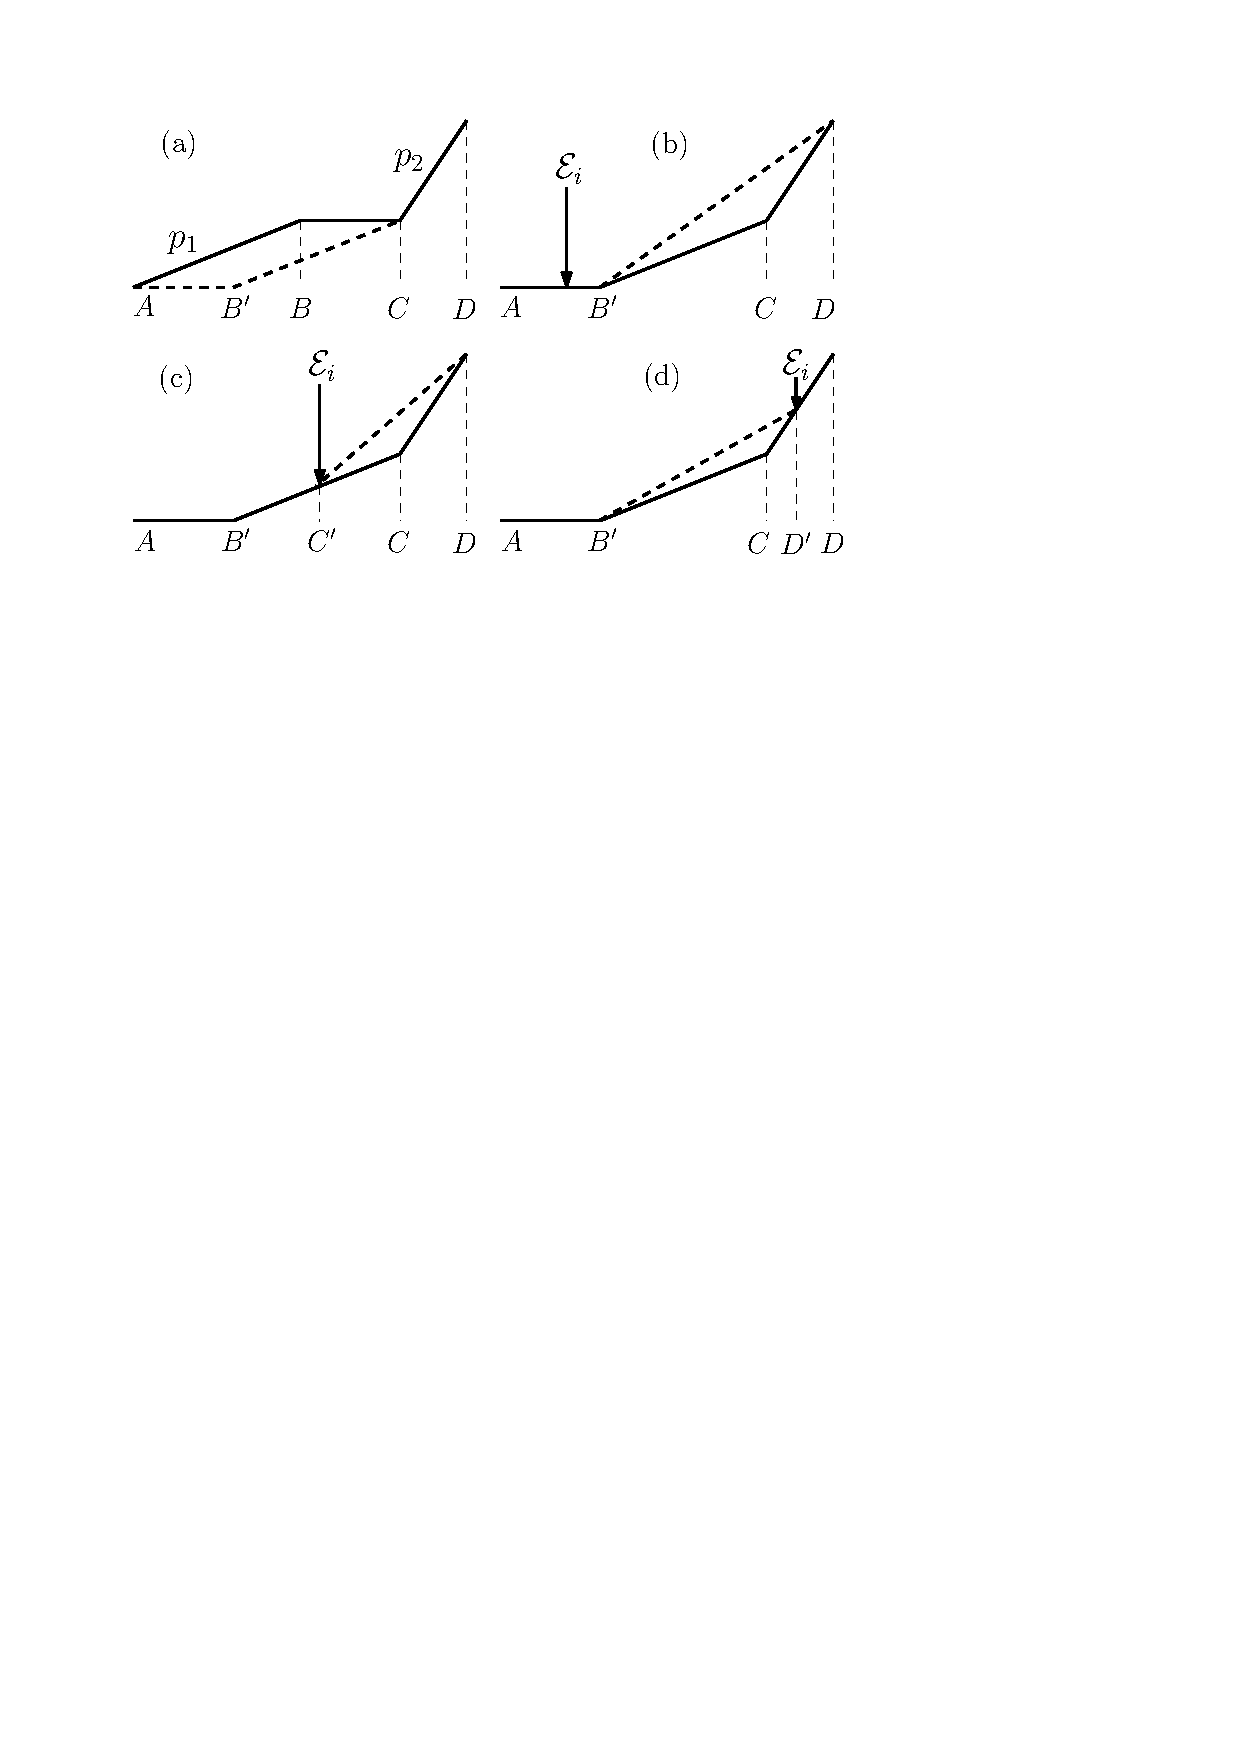
\includegraphics[width=8cm]{Lemma2.pdf}}
%\caption{Figure showing the three cases of Lemma \ref{lemma_nobreaks}, (a) the original scenario, (b) \textit{Case 1}, (c) \textit{Case 2} and (d) \textit{Case3} with $p_1>p_2$.}
%\label{Lemma2_figure}
%\end{figure}

\begin{lemma}
In an optimal solution with no breaks, the transmission power can only change at the time instants when energy arrives at the transmitter. The total energy used for transmission till that instant equals the total energy harvested upto that instant. The time instant where the transmission policy ends also satisfies this property.
\label{lemma_energy_consumed} 
\end{lemma}
\begin{proof}
Keeping in mind Lemma \ref{lemma_increasing_power} and \ref{lemma_nobreaks}, in the optimal solution $\{\textbf{p}, \textbf{s}, N\}$, transmission starts at $s_1$ and ends at $s_{N+1}$ without stopping in-between. Further, the transmission powers are also increasing. Assuming such a structure, the proof of this Lemma can be argued in similar terms of Lemma 2,3 in \cite{Yang}. 
\end{proof}	

\begin{lemma}
Consider two policies $\{\textbf{p},\textbf{s},N\}$  and $\{\bm{\widetilde{p}},\bm{\widetilde{s}},N\}$ ,which are feasible with respect to energy constraint \eqref{pb1_constraint_bits}, have non-decreasing powers and transmit same number of bits in total. If $\widetilde{p}_1=p_1-\alpha,\widetilde{p}_2=p_2,..,\widetilde{p}_{N-1}=p_{N-1},\widetilde{p}_N=p_N+\beta $ and $\widetilde{s}_1=s_1-\gamma,\widetilde{s}_2=s_2,..,\widetilde{s}_{N-1}=s_{N-1},\widetilde{s}_N=s_N+\delta $, where $\gamma=\dfrac{\alpha}{p_1-\alpha}(s_2-s_1)$, $\delta =\dfrac{\beta}{p_N+\beta}(s_{N+1}-s_N)$ and $\alpha ,\beta$ are positive constants, then 
\begin{equation}
(\widetilde{s}_{N+1}-\widetilde{s}_1)>(s_{N+1}-s_1).
\end{equation}
\label{lemma_increase_time}
\end{lemma}
\begin{proof}
The two policies $\{\textbf{p},\textbf{s},N\}$  and $\{\bm{\widetilde{p}},\bm{\widetilde{s}},N\}$ are shown in Fig. \ref{lemma4}. For every $\beta$ we can find a value of $\alpha$ such that the number of bits transmitted in policy $\{\bm{\widetilde{p}},\bm{\widetilde{s}},N\}$ remains the same as policy $\{\textbf{p},\textbf{s},N\}$. So, excluding the common parts in the transmission policy $\{\textbf{p},\textbf{s},N\}$ and $\{\bm{\widetilde{p}},\bm{\widetilde{s}},N\}$, we can equate
\begin{align}
&g(p_N)(s_{N+1}-s_N)+g(p_1)(s_2-s_1)\nonumber
\\
&=g(\widetilde{p}_N)(\widetilde{s}_{N+1}-\widetilde{s}_N)+g(\widetilde{p}_1)(\widetilde{s}_2-\widetilde{s}_1)\nonumber,
\\
&\implies (p_N+\beta)p_N\frac{\delta}{\beta}\left(\frac{g(p_N)}{p_N}-\frac{g(p_N+\beta)}{p_N+\beta}\right)\nonumber
\\
&=(p_1-\alpha)p_1\frac{\gamma}{\alpha}\left(\frac{g(p_1-\alpha)}{p_1-\alpha}-\frac{g(p_1)}{p_1}\right).\label{bits_equal}
\end{align}
$\exists$ $p_N':p_N<p_N'<p_{N}+\beta$ and $p_1':p_1-\alpha<p_1'<p_{1}$ such that
\begin{align}
&\frac{d}{dp} \frac{g(p)}{p} \bigg{\vert}_{p=p_N'}=\frac{1}{\beta}\left(\frac{g(p_N+\beta)}{p_N+\beta}-\frac{g(p_N)}{p_N}\right),\label{diff_1}
\\
&\frac{d}{dp} \frac{g(p)}{p}\bigg{\vert}_{p=p_1'}=-\frac{1}{\alpha}\left(\frac{g(p_1-\alpha)}{p_1-\alpha}-\frac{g(p_1)}{p_1}\right)\label{diff_2}.
\end{align}
Substituting (\ref{diff_1}) and (\ref{diff_2}) into (\ref{bits_equal}) we get,
\begin{align}
&\delta(p_N+\beta)p_N\frac{d}{dp} \frac{g(p)}{p}  \bigg{\vert}_{p=p_N'}
=\gamma(p_1-\alpha)p_1\frac{d}{dp} \frac{g(p)}{p} \bigg{\vert}_{p=p_1'}.\label{bits_equal1}
\end{align}
It can be verified that $\dfrac{d}{dp} \dfrac{g(p)}{p}$ is a decreasing function of $p$ using \eqref{property_concave}. As $p_1'<p_N'$, equation (\ref{bits_equal1}) implies $\gamma >\delta$. Hence the time for which transmission occurs in the policy $\{\bm{\widetilde{p}},\bm{\widetilde{s}},N\}$, $\left( s_{N+1}-s_1+\gamma-\delta\right)$, is greater than transmission time in policy $\{\textbf{p},\textbf{s},N\}$ i.e. $(s_{N+1}-s_1)$.
\end{proof}
\begin{figure}
\centering
  \centerline{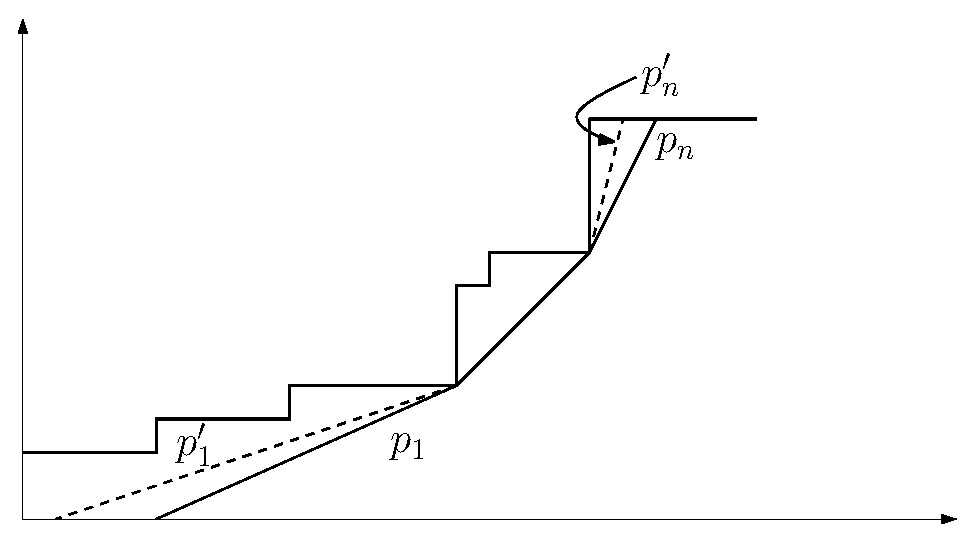
\includegraphics[width=8cm]{Lemma4.eps}}
\caption{Illustration of the proof of Lemma \ref{lemma_increase_time}.}\label{lemma4}
\end{figure}

\begin{lemma}
If the receiver has energy to stay \textit{'on'} for $\TRx_0$ time, then either the transmitter will transmit for the entire duration $\TRx_0$ or the transmitter will begin transmission at time $t=0$, in which case it stays \textit{on} for less than or equal to $\TRx_0$ time. 
\label{transmission_duration}
\end{lemma}
\begin{proof}
We will prove this by contradiction. Suppose the optimal transmission policy $\{\textbf{p},\textbf{s},N\}$ does not begin transmitting at time $t=0$ and transmits for a duration $(s_{N+1}-s_1)< \TRx_0$. Now, consider a policy $\{\bm{\widetilde{p}},\bm{\widetilde{s}},N\}$ as defined in Lemma \ref{lemma_increase_time}. By Lemma \ref{lemma_energy_consumed}, policy $\{\textbf{p},\textbf{s},N\}$ exhausts all energy at epochs $s_i$'s. So, $s_{2}$ is the first energy arrival which is on the boundary of energy constraint (\ref{pb1_constraint_energy}) i.e. $U(s_2)=\ETx(s_2^-)$ and $s_{N}$ is the last epoch satisfying $U(s_N)=\ETx(s_N^-)$. Hence we can choose $\alpha ,\beta$ such that policy $\{\bm{\widetilde{p}},\bm{\widetilde{s}},N\}$ would be feasible with respect energy constraint (\ref{pb1_constraint_energy}). By Lemma \ref{lemma_increase_time}, the time for which transmission occurs in the policy $\{\bm{\widetilde{p}},\bm{\widetilde{s}},N\}$, $\left( \widetilde{s}_{N+1}-\widetilde{s}_1\right)$, is greater than transmission time in policy $\{\textbf{p},\textbf{s},N\}$ i.e. $(s_{N+1}-s_1)$. As $s_{N+1}-s_1<\TRx_0$, we can further reduce $\alpha,\beta$ to arbitrarily small positive values so that $(s_{N+1}-s_1)<\left( \widetilde{s}_{N+1}-\widetilde{s}_1\right)<\TRx_0$ holds. With this choice of $\alpha,\beta$, policy $\{\bm{\widetilde{p}},\bm{\widetilde{s}},N\}$ is feasible with constraints  (\ref{pb1_constraint_bits}), (\ref{pb1_constraint_energy}), (\ref{pb1_constraint_time}) and contradicts the optimality of policy $\{\textbf{p},\textbf{s},N\}$ (as $\{\bm{\widetilde{p}},\bm{\widetilde{s}},N\}$ finishes before the optimal policy). This concludes that $s_{N+1}-s_1=\TRx_0$ (if $s_1\neq 0$) in optimal policy.
\end{proof}
% !TEX root = OptimalOffline.tex

Summarising the results of Lemmas \ref{lemma_increasing_power}-\ref{transmission_duration}, the optimal policy $\{\textbf{p},\textbf{s},N\}$ may change transmission powers only at energy arrival epochs i.e. $\forall 1<i<N+1,\ s_i=t_j$ for some $j$. At these epochs, it exhausts the total energy available i.e. $U(s_i)=\ETx(s_i^-)$. The transmission powers are also non-decreasing with time and the optimal policy exhausts the total `receiver time' time allowed, if it does not start transmitting from origin.

Now that we have gained some knowledge regarding the structure of the optimal policy, we consider an example to approach Problem 1. 

Suppose we are given that the receiver can be \textit{on} for a maximum duration of $\TRx_0$. Our goal is to find a transmission policy so that we can minimize the total time at which the transmission of all $B_0$ bits is completed. To do this, we shall first find a feasible solution i.e. one which satisfies all constraints (\ref{pb1_constraint_bits})-(\ref{pb1_constraint_time}) and keep improving upon it, until we have a solution that follows all structural results in Lemma \ref{lemma_increasing_power}-\ref{transmission_duration} (as shown in Theorem \ref{th_algo1_1} later,  these Lemmas form a sufficient condition as well).

We need an initial feasible solution to begin with. For this, we find the minimum energy required by the transmitter so that the transmission can be completed in duration $\TRx_0$ with a constant power. That is, the first $\ETx(t_n)$ such that
\begin{equation}
\TRx_0 g\left(\frac{\ETx(t_n)}{\TRx_0}\right)\geq B_0.
\end{equation}
Let $\widetilde{\TRx}_0\le \TRx_0$ be the time duration such that
\begin{equation}
\widetilde{\TRx}_0 g\left(\frac{\ETx(t_n)}{\widetilde{\TRx}_0}\right)=B_0.
\end{equation}
Let $p_c=\frac{\ETx(t_n)}{\widetilde{\TRx}_0}$. We try to transmit with $p_c$ power starting at time $t=0$. If it does not violate the energy constraint (\ref{pb1_constraint_energy}), we are done with the optimal solution and our transmission is completed in $\widetilde{\TRx}_0<\TRx_0$ time.

If not, we start the transmission at the earliest possible time, such that the transmission with $p_c$ for $\widetilde{\TRx}_0$ time is feasible with respect to (\ref{pb1_constraint_energy}). This transmission policy, will encounter atleast one epoch where total energy consumed till that epoch is equal to the total energy harvested upto it. Let time $t_q$ be the first point where this happens. Let $R$ and $S$ denote the starting and ending time, respectively, of transmission with power $p_c$. Clearly, $S-R=\widetilde{\TRx}_0$. This is shown in Fig. \ref{straight} (a).  Till now we have not argued why we chose such a policy to start with. In fact, Lemma \ref{lemma_Q} shows that this starting solution is a `good' estimate of policy at and before time $t_q$, as both the optimal policy and the above policy run out of all their energy at epoch $t_q$. 

Now, according to Lemma \ref{lemma_energy_consumed}, the optimal policy must finish all available energy when it stops transmission. If transmitting with $p_c$ power does use up all the energy (Fig. \ref{straight} (a)), then we accept the constant power transmission with $p_c$ as our initial policy (line number \ref{init_policy_CP} in Algorithm \ref{init_policy}). If it does not finish up all of $\ETx(t_n)$ with $p_c$ till the end of transmission (shown in Fig. \ref{straight} (b)), we choose a better policy after time $t_q$. Let $\widetilde{B}$ bits be transmitted with power $p_c$ until $S$, which is calculated in line number \ref{init_policy_bits_t_q} of procedure INIT\_POLICY in Algorithm \ref{init_policy}. Now, we require our transmission policy to send $\widetilde{B}$ bits after time $t_q$, in as little time as possible (and of course, before $S$), keeping in mind that the policy should use all $\ETx(t_n)$ amount of energy till it finishes. Algorithm 1 in \cite{Yang} does the job for us. Hence in this case, we choose transmission with $p_c$ till $t_q$ and then the solution of Algorithm 1 in \cite{Yang} after time $t_q$. 

\begin{figure}
\centering
  \centerline{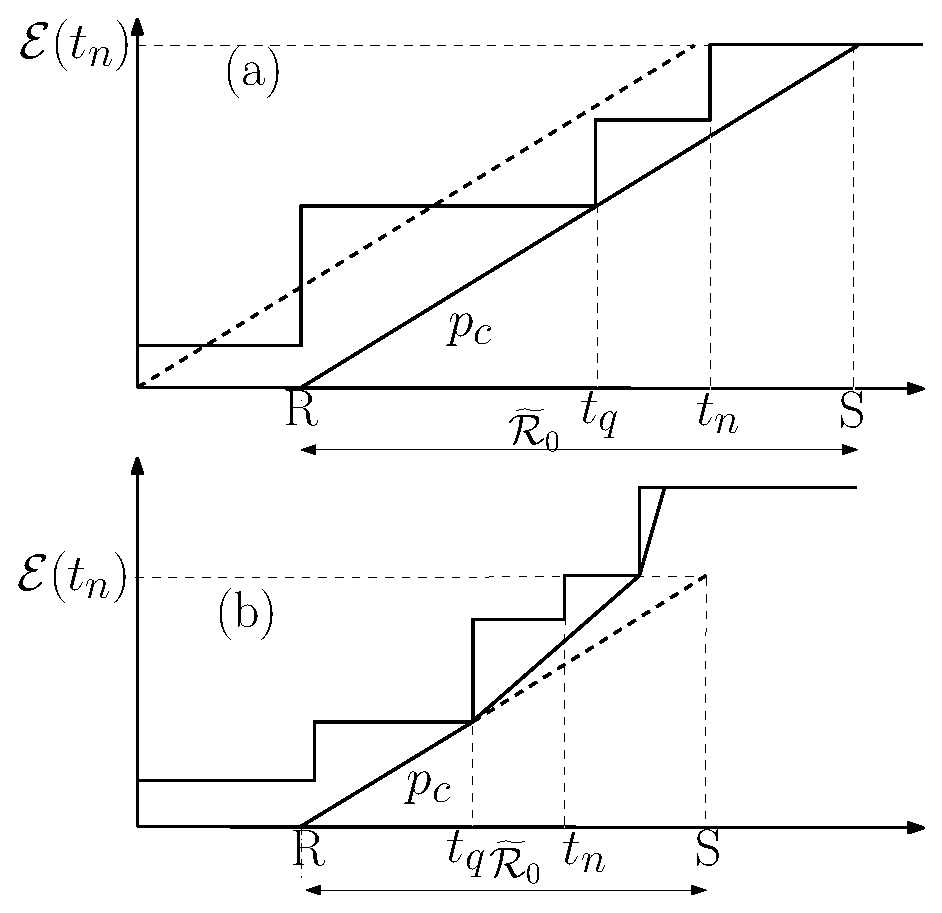
\includegraphics[width=8cm]{straight.eps}}
\caption{Figure showing point $t_q$.}\label{straight}
\end{figure}

\begin{algorithm}
%\algsetup{linenosize=\tiny}
%\alglinenumber{linenosize=\scriptsize}
\caption{Procedure to find initial feasible policy to Problem 1 for Algorithm 2}

\footnotesize%\scriptsize
\label{init_policy}
\begin{algorithmic}[1]
\State \textbf{Initialization}: $B_0$, $\TRx_0$
\Procedure{INIT\_POLICY}{}

\State $n=\displaystyle \argmin_k\left(\left\{t_k | \TRx_0 g\left(\frac{\ETx(t_k)}{\TRx_0}\right)\geq B_0\right\}\right)$ \label{init_policy_Etn}

\State Solve for $\widetilde{T}: \widetilde{T}g\left(\dfrac{\ETx(t_n)}{\widetilde{T}}\right) = B_0$\label{init_policy_CP_time}

\State $p_c=\dfrac{\ETx(n)}{\widetilde{T}}$

\State $q=\displaystyle \argmin_k\ ( \{ t_k | ((\ETx(t_k) - p_ct_k) + p_ct_j) \leq \ETx(t_j),$

$			 						\qquad \qquad \qquad \forall j\in[0,n]  \} )$
\label{init_policy_t_q}
\State $R=t_q-\dfrac{\ETx(t_q)}{p_c}$, $S=t_q+\dfrac{\ETx(t_n)-\ETx(t_q)}{p_c}$

\If {$\ETx(t_n)<\ETx(S^-)$}
	\State $\widetilde{B}=g(p_c)(S-t_q)$\label{init_policy_bits_t_q}  
	\State $\{\textbf{p},\textbf{s},N\}\gets$  Apply Algorithm 1 in \cite{Yang} to 	minimize time of
		\Statex   transmission of $\widetilde{B}$ bits  after time $t_q$ assuming	a  total of $\ETx_{q}$   
		\Statex amount of energy available at $t_q$. 
	\State\Return $\{\{p_c,\textbf{p}\},R,\textbf{s}\},N+1\}$ \label{init_policy_Yang}
	 	\Statex (Transmission with $p_c$ from $R$ to $t_q$ and then with
	 	\Statex policy $\{\textbf{p},\textbf{s},N\}$)
\Else 
	\State\Return $\{\{p_c,p_c\},\{R,t_q,S\},2\}$ \label{init_policy_CP}
\EndIf
\EndProcedure
\end{algorithmic}
\end{algorithm}



\begin{lemma}
In every optimal solution, at energy arrival epoch $t_q$, $U(t_q)=\ETx(t_q^-)$.
\label{lemma_Q}
\end{lemma}
\begin{proof}
We shall prove this by contradiction. First, we make the following claims:

\textbf{Claim 1:} Every optimal transmission policy begins transmission at or before time $R$.

Since, $S-R=\widetilde{\TRx}_0\le \TRx_0$, by Lemma \ref{transmission_duration}, if a transmission policy has to finish before $S$, it has to start before time $\max(S-\TRx_0,0) \le \max(R,0)=R$. 

%Since we are transmitting all the bits at the maximum possible power, no policy that starts after $R$ can finish before $S$. Therefore, any policy that starts after $R$ cannot be optimal.

\textbf{Claim 2:} Every optimal transmission policy ends transmission at or before time $S$.
%This follows immediately from the fact that the policy is optimal.

If it does not, then constant power policy $p_c$ finishing at $S$ will contradict its optimality.
%Let $t_q$ equal to time $t_i$ for some $i\in\mathbb{N}$. 

Suppose we have an optimal transmission policy, say $X$,$\{\bm{p},\bm{s},N\}$, that does not exhaust all its energy at time $t_q$ i.e. $U(t_q)<\ETx(t_q^-)$. Then, by Lemma \ref{lemma_energy_consumed}, it does not change its transmission power at $t_q$. Let the transmission power of $X$ be $p_{j-1}$ at $t_q$ and $p_{j-1}$ starts from $s_{j-1}$ and goes till $s_j$. Now, $s_j<S$ by \textit{Claim 2}. Further, power $p_c$ exhausts all energy by $t_q$. So,
\begin{align}
&p_c(t_q-R)=\ETx(t_q^-)\label{eqlemmaQ1}.
\end{align}
But, by constraint (\ref{pb1_constraint_energy}),
\begin{align}
&p_c(t_q-R)+p_c(s_j-t_q)\le \ETx(s_j^-),
\\
& p_c(s_j-t_q)\stackrel{(\ref{eqlemmaQ1})}{\le} \ETx(s_j^-)-\ETx(t_q^-),
\\
& p_c(s_j-t_q)< \ETx(s_j^-)-U(t_q)=p_{j-1}(s_j-t_q),
\\
& p_c<p_{j-1} .\label{eqlemmaQ2}
\end{align}
If ${j-1}= 1$, then power at $t_q$ is the first transmission power $p_1$. But then by \eqref{eqlemmaQ2}, $p_1 > p_c$. By the definition of $p_c$, we must have $s_{1} > R$, but this will contradict \textit{Claim 1}.

So ${j-1}\ge 2$, which means that the power of transmission must change at least once between $R$ and $t_q$. By Lemma \ref{lemma_energy_consumed}, $X$ has used all energy by $s_{j-1}$ and $s_{j}$ as well. So, $p_{j}(\ETx(s_{j}^-)-\ETx(s_{j-1}^-))$ is the maximum energy available between time $s_{j-1}$ and $s_{j}$. If $R<s_{j-1}$, then $p_c$ (by \eqref{eqlemmaQ2}) uses more energy, than available between $s_{j-1}$ and $s_{j}$, which is not possible. If $s_{j-1}\le R$ then $p_{j-1}$ uses more than maximum energy available (given by $p_c(t_q-R)=\ETx(t_q^-)$ ) between time $R$ and $t_q$, violating energy constraint \eqref{pb1_constraint_energy}. 

Therefore, every optimal transmission policy must use all energy till epoch $t_q$. 

%If the optimal policy does have a power higher than $p_c$ at $t_q$, then it must have the same power of transmission either from some epoch, say $t_k$, or from the beginning of transmission. If $t_k>R$, we can show that $p_c$ becomes infeasible with respect to energy constraint (\ref{pb1_constraint_energy}) at $t_k$. If $t_k<R$, $p$ becomes infeasible with energy constraint \eqref{pb1_constraint_energy} at time $R$. Now, only thing left is the optimal policy begins transmission with power $p$. If so, then it has to begin transmission after time $R$ which follows from equation (\ref{eqlemmaQ2}). This violates \textit{Claim 1}. Therefore every optimal transmission policy must use all energy till epoch $t_q$.
\end{proof}

Now that we have an initial feasible solution, we shall proceed to improve upon this policy as follows. The formal algorithm is presented as Algorithm \ref{Algorithm1}. We explain the procedure by an example. Assume that the starting feasible solution is given by the constant power policy, as shown by dotted line in Fig. \ref{figure_example_Algorithm1} (a), where $t_q=t_2$. We first assign the following initial values for the initial feasible policy - transmission power left of $t_2$ as $p_l=p_c$, power right of $t_2$ as $p_r=p_c$, start time $T_{start}=R$, stop time $T_{stop}=S$, epoch at which $p_l$ ends as $t_l=t_2$, epoch at which $p_r$ starts as $t_r=t_2$. Now, we increase $p_r$, keeping $t_r$ fixed, till it reaches $p_r'$ which hits epoch $t_3$, as shown by the solid line in Fig \ref{figure_example_Algorithm1} (a). As in total we need to transmit $B_0$ bits, the decrease in bits transferred by $p_r$ to $p_r'$ (RHS of \eqref{eq_example1}) is compensated by calculating appropriate $p_l'$ according to the following equation, where LHS represents the increase in bits transmitted from $p_l$ to $p_l'$.
\begin{align}
&g(p_l')\frac{\ETx(t_l^-)}{p_l'}-g(p_l)(t_l-T_{start})=-g(p_r)(T_{stop}-t_r)\nonumber\\
&+g(p_r')(\mathcal{P}(t_r,t_3))\frac{\ETx(T_{stop}^-)-ETx(t_r^-)}{\mathcal{P}(t_r,t_3)}.
\label{eq_example1}
\end{align}   
Having got a feasible $p_l'$, as shown in Fig. \ref{figure_example_Algorithm1} (a), we assign $T_{start}'$ with the point where $p_l'$ starts, $T_{stop}'$ with the point where $p_r'$ ends. $t_r'$ gets the value $t_3$ and $t_l'$ remains same as $t_l=t_2$. Note that parameters $\{T_{start}',T_{stop}',t_l',t_r',p_l',p_r'\}$ define the policy at the end of first iteration. 

In the next iteration, the portion of transmission between $t_l'=t_2$ to $t_r'=t_3$ is not updated. In this iteration, we try to increase $p_r'$ about $t_r'$ till it hits the feasibility equation \eqref{pb1_constraint_energy} of energy. $p_r'$ could virtually be increased to infinity. But transmission with infinite power for 0 time does not transmit any bits. So we assign $t_r''=t_2$ and $p_r''=\mathcal{P}(t_2,t_3)$. With this change in $p_r'$ to $p_r''$, we again calculate $p_l''$ which compensates the decrease in bits transferred after $t_r'$. But the calculated $p_l''$ becomes infeasible at $t_1$ as shown in Fig. \ref{figure_example_Algorithm1} (b). Hence, we set $p_l''$ to the maximum feasible power $\mathcal{P}(t_1,t_2)$ as shown in Fig. \ref{figure_example_Algorithm1} (c). With this $p_l''$, we re-calculate $p_r''$, so as to transmit $B_0$ bits in total. $t_l''$ is assigned to $t_1$, $t_r''$ remains $t_3$. $T_{start}''$ and $T_{stop}''$ as calculated to values marked in Fig. \ref{figure_example_Algorithm1} (c). The final policy at the end of second iteration is shown by solid line in Fig. \ref{figure_example_Algorithm1} (c). Like this, we continue to the third iteration, by improving the policy (to finish earlier) before $t_l''$ and after $t_r''$ and so on.


\begin{figure}
\centering
  \centerline{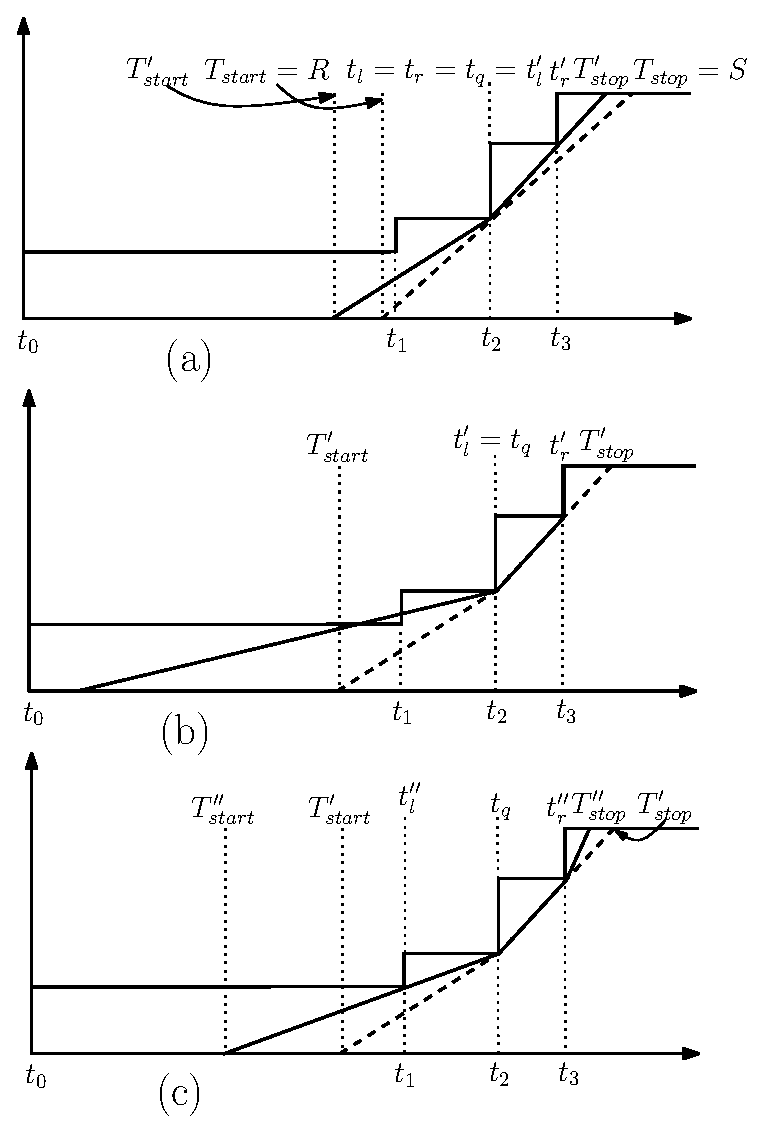
\includegraphics[width=8cm]{example_algo1.eps}}
\caption{Figures showing (a) first  and (c) second iteration of the Algorithm \ref{Algorithm1} through an example. (b) representes an intermidiate step in second iteration. In any diagram, the dashed line represent previous iteration policy and solid line is the present iteration policy.}\label{figure_example_Algorithm1}
\end{figure}


Now we describe the algorithm in steps. In any iteration, let $t_{l}$ and $t_{r}$ be the first and last energy arrival epochs where the power of transmission changes. $p_l$ and $p_r$ are the transmission power before $t_l$ and after $t_r$ respectively. $T_{start}$ and $T_{stop}$ are the start and finish time of the policy, found in any iteration. The policy found by the Algorithm in-between time $t_l$ and $t_r$ is stored in array \textbf{p} and \textbf{s}. The possible cases that can happen in an iteration of the Algorithm are shown in Fig. \ref{figure_Algorithm1}. 

Step1: The Algorithm tries to increase $p_r$ as much as possible till it hits the boundary of energy constraint \eqref{pb1_constraint_energy} as shown in Fig. \ref{figure_Algorithm1}(a). Then the Algorithm calculates the possible power $p_l'$ such that it transmits same number of bits in total with the previous iteration policy, i.e. $B_0$, as shown in line number \ref{algo_bits_left_1} and \ref{algo_bits_left_2} of Algorithm \ref{Algorithm1}. 

Step2: If $p_l'$ is feasible, which is the case shown in Fig. \ref{figure_Algorithm1}(a), the policy changes $p_l$ to $p_l'$ and $p_r$ to $p_r'$ (with $t_r$ to $t_r'$). $T_{start}$ and $T_{stop}$ are changed accordingly to start and end points of $p_l'$  and $p_r'$. 

Step3: If $p_l'$ is not feasible, as shown in Fig. \ref{figure_Algorithm1}(b), then $p_l'$ is set to be the maximum possible feasible power from $t_l$, as shown in Fig. \ref{figure_Algorithm1}(c). Now, $p_r'$ is calculated so as to settle the transmission of equal number of bits as the previous iteration. 
%We can be sure that $p_r'$ calculated now, would not be infeasible. 
In this case $t_l$ gets updated to $t_l'$.  

Going back to the first step of the algorithm where we were increasing $p_r$, it could happen, as shown in Fig. \ref{figure_Algorithm1}(d), that $p_r$ can increase to infinity without violating the energy constraint \eqref{pb1_constraint_energy}. This happens when there is no energy epoch between $t_r$ and $T_{stop}$. In this scenario, transmission is stopped at $t_r$,i.e. $T_{stop}$ gets updated to $t_r$ and both $t_r$ and $p_r$ are set to the last values in array \textbf{s},\textbf{p} receptively. This is shown in Fig. \ref{figure_Algorithm1}(d). Now, the Algorithm proceeds to calculate $p_l'$ as done in Step1, and continues as before to check whether $p_l'$ is feasible and decides according to Step2 or Step3.

\begin{figure}
\centering
  \centerline{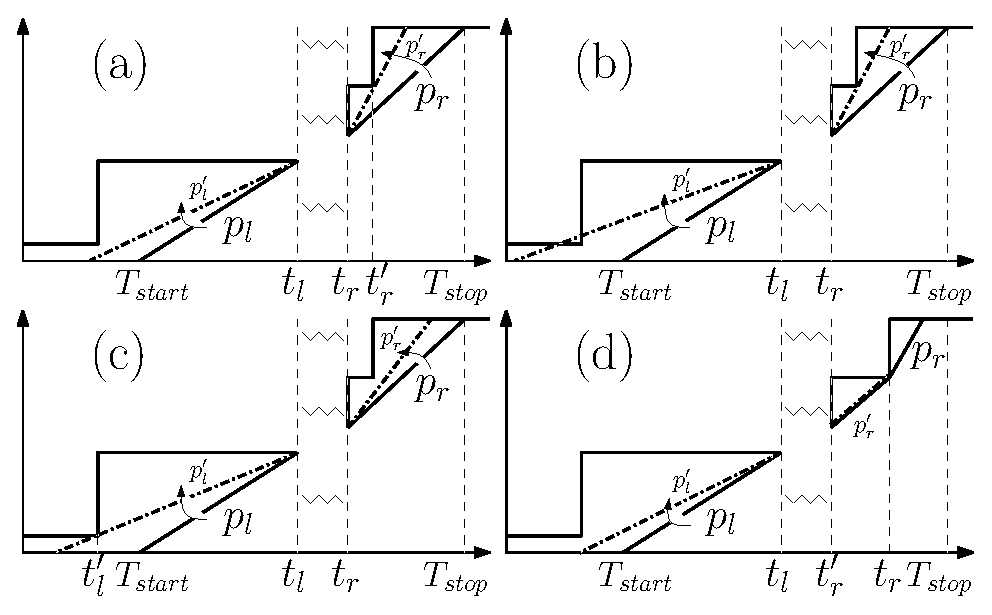
\includegraphics[width=8cm]{Algorithm1.eps}}
\caption{Figures showing any iteration of the Algorithm \ref{Algorithm1}. The solid line represents the transmission policy in the previous iteration. The dash dotted lines in (a), (b), (c), (d) represent the possible configurations of policy in the current iteration.}\label{figure_Algorithm1}
\end{figure}

This is how the algorithm proceeds to generate a new transmission policy in every iteration, which begins and ends earlier than the policy given by the previous iteration, until a point is reached where either $T_{stop}-T_{start}>\TRx_0$ or $T_{start}=0$. Suppose the Algorithm terminates with $T_{start}=0$ and $T_{start}-T_{stop}\le\TRx_0$, then the policy at this iteration is the optimal policy, as will be proved in Theorem \ref{th_algo1_2}. 


For the case where the algorithm terminates with $T_{stop}-T_{start}>\TRx_0$, let $\{T_{start}',T_{stop}',p_l',p_r',t_l',t_r'\}$ be the values in the termination iteration and $\{T_{start},T_{stop},p_l,p_r,t_l,t_r$ be the values in the previous iteration. Then, the possible valid configurations can be one of the three shown in Fig. \ref{figure_Algorithm1} (a) (c) (d). Note that $\ETx(T_{stop}^-)=\ETx(T_{stop}'^-)$ in all the cases. (In case Fig. \ref{figure_Algorithm1} (d) we can assume that $T_{stop}'=t_r^+$ and transmission exists after $t_r$, but with infinite power. Since transmitting with infinite power for $0$ time does not transmit any bits, we would transmit the same number of bits, as we did prior to this modification). Thus, by Lemma \ref{lemma_increase_time}, we can verify that $(T_{stop}'-T_{start}')>(T_{stop}-T_{start})$. Since $(T_{stop}'-T_{start}')>\TRx_0>(T_{stop}-T_{start})$, there must exist a solution to equation presented in line number \ref{algo_solve_eqn} of Algorithm \ref{Algorithm1}. Let the policy obtained from the solution start and end at $T_{start}''$ and $T_{stop}''$. Then $T_{stop}''$ and $T_{start}''$ would lie in-between $T_{stop}$,$T_{stop}'$ and $T_{start}$,$T_{start}'$ respectively. Also, $T_{stop}''-T_{start}''=\TRx_0$.

So we can conclude by stating that, the solution to Algorithm \ref{Algorithm1} satisfies Lemma \ref{transmission_duration}. Now, according to the definition of $t_n$ and $t_q$ in line number \ref{init_policy_Etn} and \ref{init_policy_t_q} of INIT\_POLICY, $t_q\le t_n$ and $\ETx(t_q)<\ETx(t_n)$. Since $t_n$ is defined as the first energy arrival epoch by which $B_0$ bits can be transmitted in $\TRx_0$ time, any transmission policy which ends at or before $t_n$ should take more than $\TRx_0$ time to transmit all of $B_0$ bits. As $t_q\le t_n$, we are guaranteed that no transmission policy can finish at or before $t_q$. Hence in the iterations of the algorithm $t_r$ can never decrease beyond $t_q$. As $t_q$ is present in the initial solution, $t_q$ always exists in the final solution to Algorithm \ref{Algorithm1}.   

%!TEX root = OptimalOffline.tex
%input{Siddhartha}
\begin{theorem}
Let a transmission policy to solve Problem 1 is given by power vector $\textbf{p}=[p_1,p_2,..,p_N]$ and the start time of transmission for the corresponding power be given by vector $\textbf{s}=[s_1,s_2,..,s_N]$, for some $N\in \mathbb{N}$. The transmission ends at time $s_{N+1}$. Now such a policy is optimal if and only if it satisfies the following structure.
\label{th_algo1_1}
\begin{align}
&\sum_{i=1}^{i=N}g(p_i)(s_{i+1}-s_i)=B_0\label{claim1}
\\
&\nonumber s_{N+1}-s_1=T^R_0 				&&\text{ , if } s_1>0
\\
& \text{ or } s_{N+1}\le T^R_0 				&&\text{ , if } s_1=0\label{claim2}
\\
&\nonumber s_{n+1}=\argmin_{t_i: s_n < t_i \le s_{N+1}} CP(t_i,s_n)
\\
&\text{ and } p_n=CP(s_{n+1},s_n)\label{claim3}
\\
&\exists s_j:s_j\in \textbf{s} \text{ and } s_j=Q\label{claim4}
\end{align}
for $n=\{ 1,2,..,N-1\}$.
\end{theorem}
\begin{proof}
First we show that the optimal policy should have the given structure. The proof follows the method of  contradiction. We establish structure (\ref{claim3}) at first. Assume an optimal policy that satisfies Lemmas 1 to 6 and does not satisfy the given structure (\ref{claim3}). Specifically, say the policy be same as structure (\ref{claim3}) from time $s_{1}$ to $s_n$, for some $n\in \{1,2,..,N\}$ but transmission power right after $s_n$ is not the minimum feasible constant power, i.e.
\begin{align}
p_n>CP(s',s_n)\text{ where } s'=\argmin_{t_i: s_n < t_i \le s_{N+1}} CP(t_i,s_n)\label{claim3_1}
\end{align}

\textit{Case1: }if $s'>s_{n+1}$ for some $n\in \{1,2,..,N-1\}$, then the energy that is used for transmission from time $s'$ to $s_{n+1}$ is given by $\ETx(s'-)-\ETx(s_{n+1}^-)$ in terms of Lemma 3. We claim that that there must be a time duration from $s'$ to $s_{n+1}$ for which the transmission power is less than $p_n$. If this claim is true then we violate lemma \ref{increasing_power} and hence contradict the assumption. Coming to the claim, if it does not hold i.e. transmission power at all points of time between $s_{n+1}$ to $s'$ is more than $p_n$, then the total energy used during this period can be lower bounded by $p_n(s'-s_{n+1})$. Next, we show that this energy is more that what is harvested during $s_{n+1}$ to $s'$ making it infeasible. As transmitting with $CP(s',s_n)$ power is a feasible between time $s'$ and $s_n$, $CP(s',s_n)(s_{n+1}-s_n)\le \ETx(s_{n+1}^-)-\ETx(s_{n}^-)$. So, 
\begin{align}
&\ETx(s'-)-\ETx(s_{n+1}^-) \le \ETx(s'-)-\ETx(s_{n+1}^-)
\\
&+(\ETx(s_{n+1}^-)-\ETx(s_{n}^-)-CP(s',s_n)(s_{n+1}-s_n))
\\
&=CP(s',s_n)(s'-s_{n+1})\stackrel{(\ref{claim3_1})}{<}p_n (s'-s_{n+1}).
\end{align}

\textit{Case2: }if $s'<s_{n+1}$, the transmission policy uses $p_n(s'-s_{n})$ energy from time $s_n$ to $s'$. But $\ETx(s'-)-\ETx(s_{n}^-)=CP(s',s_n)(s'-s_{n})\stackrel{\ref{claim3_1}}{<}p_n(s'-s_{n})$. So, energy used $p_n(s'-s_{n})$ is more than what is harvested making this case infeasible.

%Note that equation (\ref{claim1}) must be followed by the optimal policy as it is a constraint to the optimization problem 1. We move on to prove structure (\ref{claim2}). If $s_1=0$ then $s_{N+1}$ has to be less than or equal to $T^R_0$ due to constraint 1. When $s_1>0$, assume that $s_{N+1}-s_1<T^R_0$. Let $A$ be the first energy arrival such that $E(A)=\ETx(A^-)$. Similarly, let $B$ be the last energy arrival at which $E(B)=\ETx(B^-)$. Now consider the policy where power vector is given by $\{p_1-\alpha,p_1,p_2,..,p_{N-1},p_N,p_N+\epsilon \}$ and the corresponding time vector be given by $\{s_1-\beta,A,s_2,..,s_{N},B\}$ with the transmission ending at time $s_{N+1}-\gamma$, where $\epsilon$ is a small positive constant, $\beta=\frac{\alpha}{p_1-\alpha}(A-s_1) $, $\gamma= \frac{\epsilon}{p_N+\epsilon}(s_{N+1}-B)$. This policy finishes before the previous policy and hence contradicts its optimality only if we are able to show that it is feasible. Such a policy would be feasible with respect to the energy constraint keeping in mind that transmission with power $p_N+\epsilon $ from time $A$ to $s_{N+1}-\gamma$ was previously never on the boundary of feasibility constraint 1 and similarly for power $p_1-\alpha $. Now we see its feasibility with constraint 2. For every $\epsilon \rightarrow 0^{+}$ we can find a value of $\alpha$ such that the number of bits transmitted in this new policy remains the same as the previous one i.e. $B_0$. So, excluding the common terms from equating the number of bits boils to
%\begin{align}
%&\nonumber g(p_N)(s_{N+1}-B)+g(p_1)(A-s_1)
%\\
%&\nonumber =g(p_1-\alpha)(A-s_1+\beta)+g(p_N+\epsilon)(s_{N+1}-B-\gamma)
%\\
%&\nonumber\implies (s_{N+1}-B)(g(p_N)-g(p_N+\epsilon)\frac{p_N}{p_N+\epsilon})
%\\
%&=(A-s_1)(g(p_1-\alpha)\frac{p_1}{p_1-\alpha}-g(p_1))\label{bits}
%\end{align} 
%Now the total time for which the transmission is \textit{on} is $s_{N+1}-s_1+\beta-\gamma$.


Note that equation (\ref{claim1}) must be followed by the optimal policy as it is a constraint to the optimization problem 1. We move on to prove structure (\ref{claim2}). If $s_1=0$ then $s_{N+1}$ has to be less than or equal to $T^R_0$ due to constraint 1. When $s_1>0$, assume that $s_{N+1}-s_1<T^R_0$. Let $A$ be the first energy arrival such that $E(A)=\ETx(A^-)$. Similarly, let $B$ be the last energy arrival at which $E(B)=\ETx(B^-)$. Now consider the policy where power vector is given by $\{p_1+dp_1,p_1,p_2,..,p_{N-1},p_N,p_N+dp_N \}$ and the corresponding time vector be given by $\{s_1+ds_1,A,s_2,..,s_{N},B\}$ with the transmission ending at time $s_{N+1}+ds_{N+1}$, where $dp_N>0$ and  $dp_1,ds_1, ds_{N+1}<0$ . This policy finishes before the previous policy and hence contradicts its optimality only if we are able to show that it is feasible. Such a policy would be feasible with respect to the energy constraint keeping in mind that transmission with power $p_N$ from time $A$ to $s_{N+1}$ was previously never on the boundary of feasibility constraint 1 and similarly for power $p_1$. Now we see its feasibility with respect to constraint 2. It can be seen that
\begin{align}
&p_1ds_1=(A-s_1)dp_1\text{ , }p_Nds_{N+1}=-(s_{N+1}-B)dp_N
\end{align}
The number of bits transmitted from time $s_1$ to $A$ is given by $B_1=g(p_1)(A-s_1)$ and similarly, from $B$ to $s_{N+1}$ be given by $B_N=g(p_N)(s_{N+1}-B)$ under the previous policy. Noting that the number of bits sent in the two policies remains same we get,
\begin{align}
&\nonumber dB_1+dB_2=0
\\
&\nonumber\implies g'(p_1)(A-s_1)dp_1-g(p_1)ds_1
\\
&\nonumber +g'(p_N)(s_{N+1}-B)dp_N+g(p_N)ds_{N+1}=0
\\
&\nonumber\implies \frac{-ds_1}{-ds_{N+1}}=\frac{(g'(p_N)p_N-g(p_N))}{(g'(p_1)p_1-g(p_1)}
\end{align}
We can verify that $g'(p)p-g(p)$ is an increasing function of $p$ for $p>0$ due to concavity of $g(p)$. Hence $(-ds_1)\ge (-ds_{N+1})$. The time for which transmission is on in this policy is $s_{N+1}-s_1+ds_{N+1}-ds_1\ge s_{N+1}-s_1$. As $s_{N+1}-s_1<T^R_0$, we can choose arbitrarily small negative value of $ds_{N+1}$ so that $s_{N+1}-s_1\le s_{N+1}-s_1+ds_{N+1}-ds_1<T^R_0$ holds. So the new policy finishes earlier than the previous policy contradicting the optimality. This concludes that $s_{N+1}-s_1=T^R_0$ (if $s_1\neq 0$) in optimal policy.

Next, we prove the sufficiency of the structure. Let the power vector $\textbf{p}$ and time vector $\textbf{s}$ follow the structure. We need to show that this policy is optimal. Assume that there exists another policy given by $\{\textbf{p'},\textbf{s'}\}$ which abides by the Lemma 1-5 and is optimal, but does not follow the structure. We argue next that such a policy is not feasible and hence contradict its optimality. 

\textit{Case1}: If $s_1'>s_1\ge 0$ then by Lemmma  $s_{N'+1}'>s_{N+1}$. So policy $\{\textbf{p'},\textbf{s'}\}$ cannot be optimal. 

\textit{Case2}: Suppose $s_1'=s_1$. Let $s_i'$ be the first epoch for which $p_i'\ne p_i$ for some $i \in \{1,2,..,N\}$. By (\ref{claim3}), $p_i'>p_i$. If $s_{N'+1}'>s_{i+1}$, then the amount of energy used by policy $\{ \textbf{p'},\textbf{s'}\}$ in interval $[s_{i},s_{i+1}]$ is more than policy $\{\textbf{p},\textbf{s}\}$. But by Lemma, $\{\textbf{p},\textbf{s}\}$ uses all energy available by $s_{i+1}$. So policy $\{\textbf{p'},\textbf{s'}\}$ is not feasible with respect to the energy constraint. If $s_{N'+1}'\le s_{i+1}$, then it can be easily verified by property P4 that policy $\{\textbf{p'},\textbf{s'}\}$ transmits strictly less number of bits in interval $[s_i,s_{N'+1}]$ than the other policy in interval $[s_{i},s_{i+1}]$. Both policies being same till $s_i$, we conclude that policy $\{\textbf{p'},\textbf{s'}\}$ transmits less than $B_0$  bits and therefore it is not optimal.

\textit{Case3}: This case argues the infeasibility when $s_1'<s_1$. Unlike other cases this case is more rigorous. The idea of the proof is to show that if we start our transmission early and finish earlier than policy $\{\textbf{p},\textbf{s}\}$, we always take more transmission time which is going to violate the time constraint. First, we establish that the policy $\{\textbf{p'},\textbf{s'}\}$ must be same as policy $\{\textbf{p},\textbf{s}\}$ from epoch $s_2$ to an epoch $s_j$ such that $s_j=\max_{s_i<s_{N'+1}'} s_i$. Let $s_k'=max_{s_i'<s_2}s_i'$ and transmission continues with constant power $p_k'$ till $s_l'$. If $s_l'>s_2$, then transmission with a constant power $\dfrac{\ETx(s_l^{,-})}{(s_l'-s_1)} $ from $s_1$ to $s_l'$ is feasible and $\dfrac{\ETx(s_l^{,-})}{(s_l'-s_1)}<\dfrac{\ETx(s_2^-)}{(s_2-s_1)}=p_1$. This contradicts $\ref{claim3}$. So, $s_l'=s_2$. Now, if $p_l'>p_2$ and $s_j>s_3$, then the amount of energy used by policy $\{\textbf{p'},\textbf{s'}\}$ between $s_2$ and $s_3$ is more than what is harvested. So $p_l'=p_2$ ($s_{l+1}=s_3$) and similarly we can show that $p_{l+1}=p_3$.. ($ s_{l+2}=s_4$..) till epoch $s_j$. By Lemma and (\ref{claim4}) we can be sure that there exists atleast one epoch $s_i$ which belongs to $\textbf{s}$ as well as $\textbf{s'}$ i.e. $j\ge 2$.

Now, consider the following process which creates child feasible policies from policy $\{\textbf{p'},\textbf{s'}\}$. We define two pivots $pv_1$ and $pv_2$. Initially we set $pv_1=s_2'$ and $pv_2=s_{N'}'$. The transmission power right before $pv_1$ is $u$ ($u=p_1'$ initially) and right after $pv_2$ is $v$ ($v=p_{N'}'$ initially). Keeping the policy same from $pv_1$ to $pv_2$ we increase $u$ by a small amount to $u+du$ and decrease $v$ by a small amount to $v-dv$ so that the number of bits transmitted( i.e. $B_0$) remains same under this transformation. Let $s_1'$ change to $s_1'+x$ and $s_{N'+1}'$ change to $s_{N'+1}'+y$ for some $x,y>0$. Following the argument provided while proving the necessary statement of this Theorem, we can conclude that $x>y$ and hence. We denote such a policy by vectors $\{\textbf{p'(x)},\textbf{s'(x)}\}$. Note that $(s_{N'(x)+1}'(x)-s_1'(x))<(s_{N'+1}'-s_1')$. We continue increasing $x$ till either $u=p_2$ (in which case we change $pv_1=s_2$) or $v=p_{N'-1}'$ (where we change $pv_2=s_{N'-1}'$) or $s_{N'(x)+1}'(x)$ hits a epoch, say $t_j$ ($pv_2=t_j$, $v\rightarrow\infty$ in this case). After this, we again start increasing $x$ with changed definitions. We continue this process till $x=s_1-s_1'$  or $u$ becomes equal to $v$. Note that the former stopping criteria will be met at a smaller $x$ than the later one since policy $\{\textbf{p'(x)},\textbf{s'(x)}\}$ shares at least one epoch with policy $\{\textbf{p'},\textbf{s'}\}$ by arguments of previous paragraph. By maintaining these rules we ensure that policy $\{\textbf{p'(x)},\textbf{s'(x)}\}$ abides by Lemma 1-6 and is feasible with energy constraint. Since $s_{N'(x)+1}'(x)-s_1'(x)$ is decreasing with $x$, the policy is also feasible with time constraint. As this is a continuous function on $x$, at $x=s_1-s_1'$ we reach a policy such that $s_1'(x)=s_1$. At $x=s_1-s_1'$, if $s_{N'(x)+1}'(x)\ge s_{N+1}$ then $s_{N'+1}'-s_1'>s_{N'(x)+1}'(x)-s_1'(x)\ge T^R_0$ and policy $\{\textbf{p'},\textbf{s'}\}$ is infeasible with time constraint. If $s_{N'(x)+1}'(x)< s_{N+1}$ then we can follow the arguments in \textit{Case2} to show that policy $\{\textbf{p'(x)},\textbf{s'(x)}\}$ is infeasible, which in turn accounts for the infeasibility of policy $\{\textbf{p'},\textbf{s'}\}$.
\end{proof}

























%input{Rushil}
\begin{theorem}
The policy described by the above algorithm is optimal.
\end{theorem}
\begin{proof}
To prove that our policy is optimal, we have to show that it is of the structure described in the previous theorem. \\
That is, $s_{stop} - s_0 \leq T$ and \\
\textbf{Things to write}\\
First we prove that the power allocations in this algorithm are in accordance with \textbf{insert}\\
In the first part of the algorithm, we select the maximum slope at a corner point before $s_{left}$ and after $s'_{start}$ and ending at $s_{left}$. \\
First we try to show that this is also the maximum such slope between any corner point before $s_{left}$ and after $s_{start}$ where $s_{start}$ is the final start point. \\
Suppose it is not. Then we have a corner point between $s_{start}$ and $s'_{start}$ such that we can transmit with a power higher than our maximum between these two points. But, if this were possible, then 
$p_{left}$ itself would have been feasible, which is not the case. (See figure).\\
Now we seek to show that this procedure of selecting maximum slopes going 'backwards' also gives us the minimum slopes going 'forwards', as described in \textbf{insert}.\\
We shall show this by contradiction. Let $s_i$, $s_j$ and $s_k$ be three consecutive corner points where the power of transmission increases, as per our allocation. Now suppose, it is possible to transmit with a lowe power between $s_i$ and some $s'_j$. 
Then the power of transmission between $s_j$ and $s_k$ is not the maximum power since we could transmit at a higher power from $s'_j$ and $s_k$. Which is a contradiction as this is not consistent with out allocation algorithm.\\
Therefore, the allocation policy before point $Q$ is consistent with \textbf{insert}. (See figure)
We can prove similarly for the powers after point $Q$.
\end{proof}





% !TEX root = OptimalOffline.tex
\begin{table}
\begin{minipage}[b]{8cm}
\caption {Offline algorithm for energy arrival in receiver after time t=0}
\begin{tabular}{p{7cm}}
\hline \textbf{Input}: Bits to transmit $B_0$; $\ETx_i$, $\TRx_i$ for all $i$
\\
\hline
\\
\textbf{Initialize:}
\\ 
$u=\min u_i$ s.t. $\TRx(u_i)g\left( \dfrac{\ETx(u_i)}{\TRx(u_i)} \right) \ge B_0$. $O_f=\infty$.
\\
For all $i$, define $O_i=\min$ $t$ s.t. receiver can be \textit{on} from $t$ to $(t+\TRx(r_i))$, i.e. $K(x) \le \TRx(x)$,  $t \le x\le (t+\TRx(r_i))$. 
\\
\\
\textbf{if} $u=r_j$ for some $j$  \textbf{then}
\\
\hspace{4mm}$O_l=O_{j}$, $T=\TRx(r_j)$
\\
\textbf{else}
\\
\hspace{4mm}Let $u=t_j$ for some $j$
\\
\hspace{4mm}$u_{j'}=\min r_i$ s.t. $\TRx(r_i)g\Bigg{(} \dfrac{\ETx(t_j)}{\TRx(r_i)}\Bigg{)}\ge B_0$
\\
\hspace{4mm}$O_l=O_{j'}$, $T=\TRx(r_{j'})$.
\\
\textbf{end if}
\\
\textbf{do}
\\
\hspace{4mm}Apply $Algo1(O,T)\rightarrow T_{opt}$
\\
\hspace{4mm}$r_k=\max_i r_i $ s.t. $r_i<T_{opt}$ 
\\
\hspace{4mm}\textbf{if} $O_{f} > O_{k}$
\\
\hspace{7mm}$O_{f} = O_{k}$
\\
\hspace{4mm}\textbf{end if}
\\
\hspace{4mm}$l=l+1$
\\
\textbf{while} $O_l \le O_{f}$
\\
\hline
\label{online}
\end{tabular}
\end{minipage}
\end{table}
